%%=============================================================================
%% Google AutoML
%%=============================================================================

\chapter{Google Cloud AutoML}
\label{ch:google-automl}

Google Cloud AutoML is zoals de naam zegt, deel van het Cloud platform. In dit hoofdstuk wordt gebruik gemaakt van een \textit{storage server} en de \textit{vision API}. Om toegang te krijgen is uiteraard een account nodig, en als nieuwe gebruiker is er \$300 beschikbaar die vrij gespendeerd kan worden op het platform (binnen de periode van één jaar).

De interfaces zijn zeer gebruiksvriendelijk en maken vaak gebruik van drag en drop systemen. 

Vooraleer er gestart kan worden is een korte setup op zijn plaats. De volledige code van het gebruikte \textit{jupyter notebook} is te vinden in Appendix \ref{ch:app:google-automl}.

\section{Voorafgaand werk}
\label{sec:google-automl-before}

\subsection{Google Cloud Data Storage}
\label{subsec:google-cloud-data-storage}

Om de \textit{computer vision API} te gebruiken moeten de afbeeldingen geüpload worden. Dit kan rechtstreeks in batches van max. 30 MB. Met de hoeveelheid afbeeldingen die gebruikt worden in dit onderzoek is dit niet praktisch. Voor grote hoeveelheden data kan daarom een online bucket gebruikt worden. De afbeeldingen bevinden zich dan op een \textit{data storage server} van Google Cloud.

De indeling van de data moet er als volgt uitzien:

\dirtree{%
    .1 online bucket.
    .2 cat.
    .3 cat.0.jpg.
    .3 cat.1.jpg.
    .3 cat.2.jpg.
    .2 dog.
    .3 dog.0.jpg.
    .3 dog.1.jpg.
    .3 dog.2.jpg.
}

Dit is belangrijk voor de volgende stap. Op deze manier kunnen er makkelijk labels toegekend worden aan de afbeeldingen. Dit op een manier die het platform kan interpreteren.

\subsection{Structuur van de data}
\label{subsec:google-structure}

Nu alle data online beschikbaar is, moet er nog een overzicht gecreëerd worden. Aan de hand van een \textit{jupyter notebook} wordt een csv gemaakt die voor elke afbeelding, de locatie op Google Cloud Storage en het bijhorend label bevat. Alle niet afbeeldingen worden uit de map gefiltered

\begin{python}
data_array = []

for (dict_key, files_list) in files_dict.items():
    for filename in files_list:
        if '.jpg' not in filename:
            continue # don't include non-photos
            
        label = dict_key
        data_array.append((base_gcs_path + dict_key + '/' + filename , label))

\end{python}

Nu moet \pyth{data_array} enkel nog ingeladen worden in een \textit{pandas dataframe}. In de \textit{pandas library} zit een functie die een dataframe kan opslaan als een csv bestand. Merk op dat de indexes van de kolommen en rijen niet mee opgeslagen worden. Deze kunnen als \pyth{False} geflagged worden in de functie.

\pyth{dataframe.to_csv('all_data.csv', index=False, header=False)}

De output van het csv bestand zou er als onderstaand uit moeten zien. Natuurlijk met een andere bucket naam.

gs://rdc-automl-catsvsdogs/dog/dog.100.jpg dog \\
gs://rdc-automl-catsvsdogs/dog/dog.1000.jpg dog \\
… … … \\
gs://rdc-automl-catsvsdogs/cat/cat.9995.jpg cat \\
gs://rdc-automl-catsvsdogs/cat/cat.9996.jpg cat
\\

Het csv bestand moet dan ook toegevoegd worden aan de bucket.

\section{Model trainen en evalueren}
\label{sec:google-automl-train}

Om het trainen te starten moet nu enkel het csv bestand (dat op Google Cloud Storage) staat selecteren. Vervolgens worden alle afbeeldingen geïmporteerd en opgesplitst in training, validatie en testen. In ons geval van 25000 afbeeldingen worden ze als volgt opgesplitst.

\begin{itemize}
    \item Training: 10000
    \item Validatie: 5000
    \item Testen: 5000
\end{itemize}

Elke dataset is gelijk verdeeld over de twee categorieën. Als er dus over 10000 afbeeldingen gesproken worden, zijn het in feite 5000 katten en 5000 honden.

\section{Model visualisatie}
\label{sec:google-automl-visualisation}

\section{Deployment}
\label{sec:google-automl-deployment}

Zoals besproken in sectie \ref{subsubsec:client-library} kunnen er interacties zijn via een \textit{client library}. De code kan oftewel intern in de applicatie verwerkt worden (indien de code geschreven is in Python). Een tweede manier is om de het Python script extern op te slaan en op te roepen als het nodig is.

\bigskip

\begin{python}
import sys

from google.cloud import automl_v1beta1
from google.cloud.automl_v1beta1.proto import service_pb2


# 'content' is base-64-encoded image data.
def get_prediction(content, project_id, model_id):
    prediction_client = automl_v1beta1.PredictionServiceClient()
    
    name = 'projects/{}/locations/us-central1/models/{}'.format(project_id, model_id)
    payload = {'image': {'image_bytes': content }}
    params = {}
    request = prediction_client.predict(name, payload, params)
    return request  # waits till request is returned

if __name__ == '__main__':
    file_path = sys.argv[1]
    project_id = sys.argv[2]
    model_id = sys.argv[3]

    with open(file_path, 'rb') as ff:
        content = ff.read()
    
    print get_prediction(content, project_id, model_id)
\end{python}

De functie verwacht drie argumenten. Een afbeelding (geëncodeerd in base-64), het project\_id en het model\_id. De ID's zijn te vinden in de eigenschappen van het project en model op Google Cloud.

\bigskip

\begin{python}
python predict.py YOUR_LOCAL_IMAGE_FILE 156243918112 ICN8843552342109323264
\end{python}

\begin{figure}
    \centering
    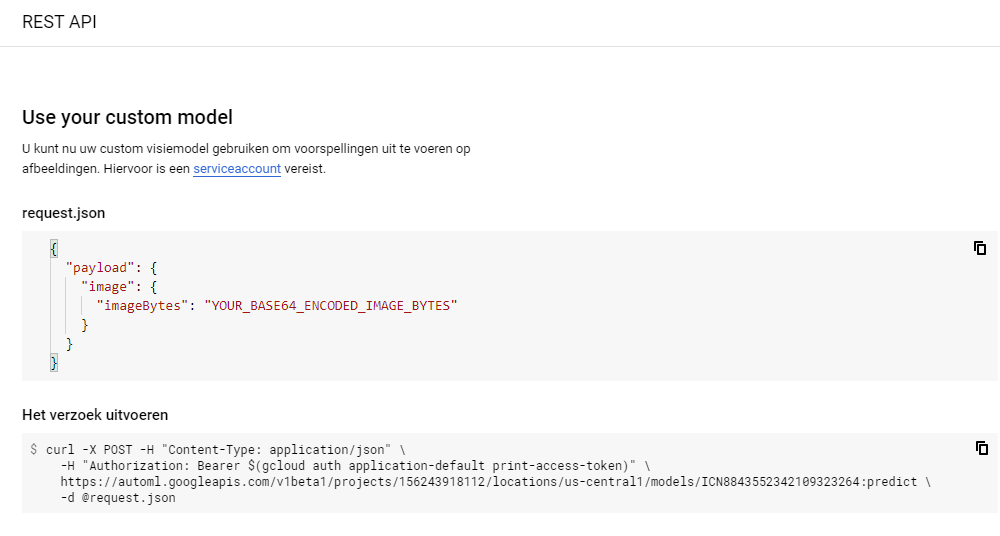
\includegraphics[width=\linewidth]{img/google-automl-rest.png}
    \caption{Requests sturen naar de REST API van Google AutoML.}
    \label{fig:google-automl-rest}
\end{figure}

Als een model gedeployed is, wordt er standaard een REST service aangemaakt. De gebruiker kiest dan zelf om een wrapper te schrijven (om een familiaire interface te maken) of om de requests met curl door te sturen, zoals op afbeelding \ref{fig:google-automl-rest}. 


\section{Requirements}
\label{sec:google-requirements}